\section{Methods}
\label{sec:methods}

We create and analyze cell class-specific connectivity matrices using models trained on murine viral-tracing experiments.
This section describes the data used to generate the model, the model itself, the evaluation of the model, and the use of the model in creation of the connectivity matrices.
It also includes background on the non-negative matrix factorization method used for decomposing the wild-type connectivity matrix into latent structures.
Additional information on our data is given in Supplemental Section \ref{supp_sec:data} methods is given in Supplemental Section \ref{supp_sec:methods}.

\newpage
\begin{figure}[H]
\subfloat[]{
\label{fig:mouse}
    
\includegraphics[width=0.3\textwidth]{figs/figure1a.png}}
\subfloat[]{
\label{fig:injproj}
    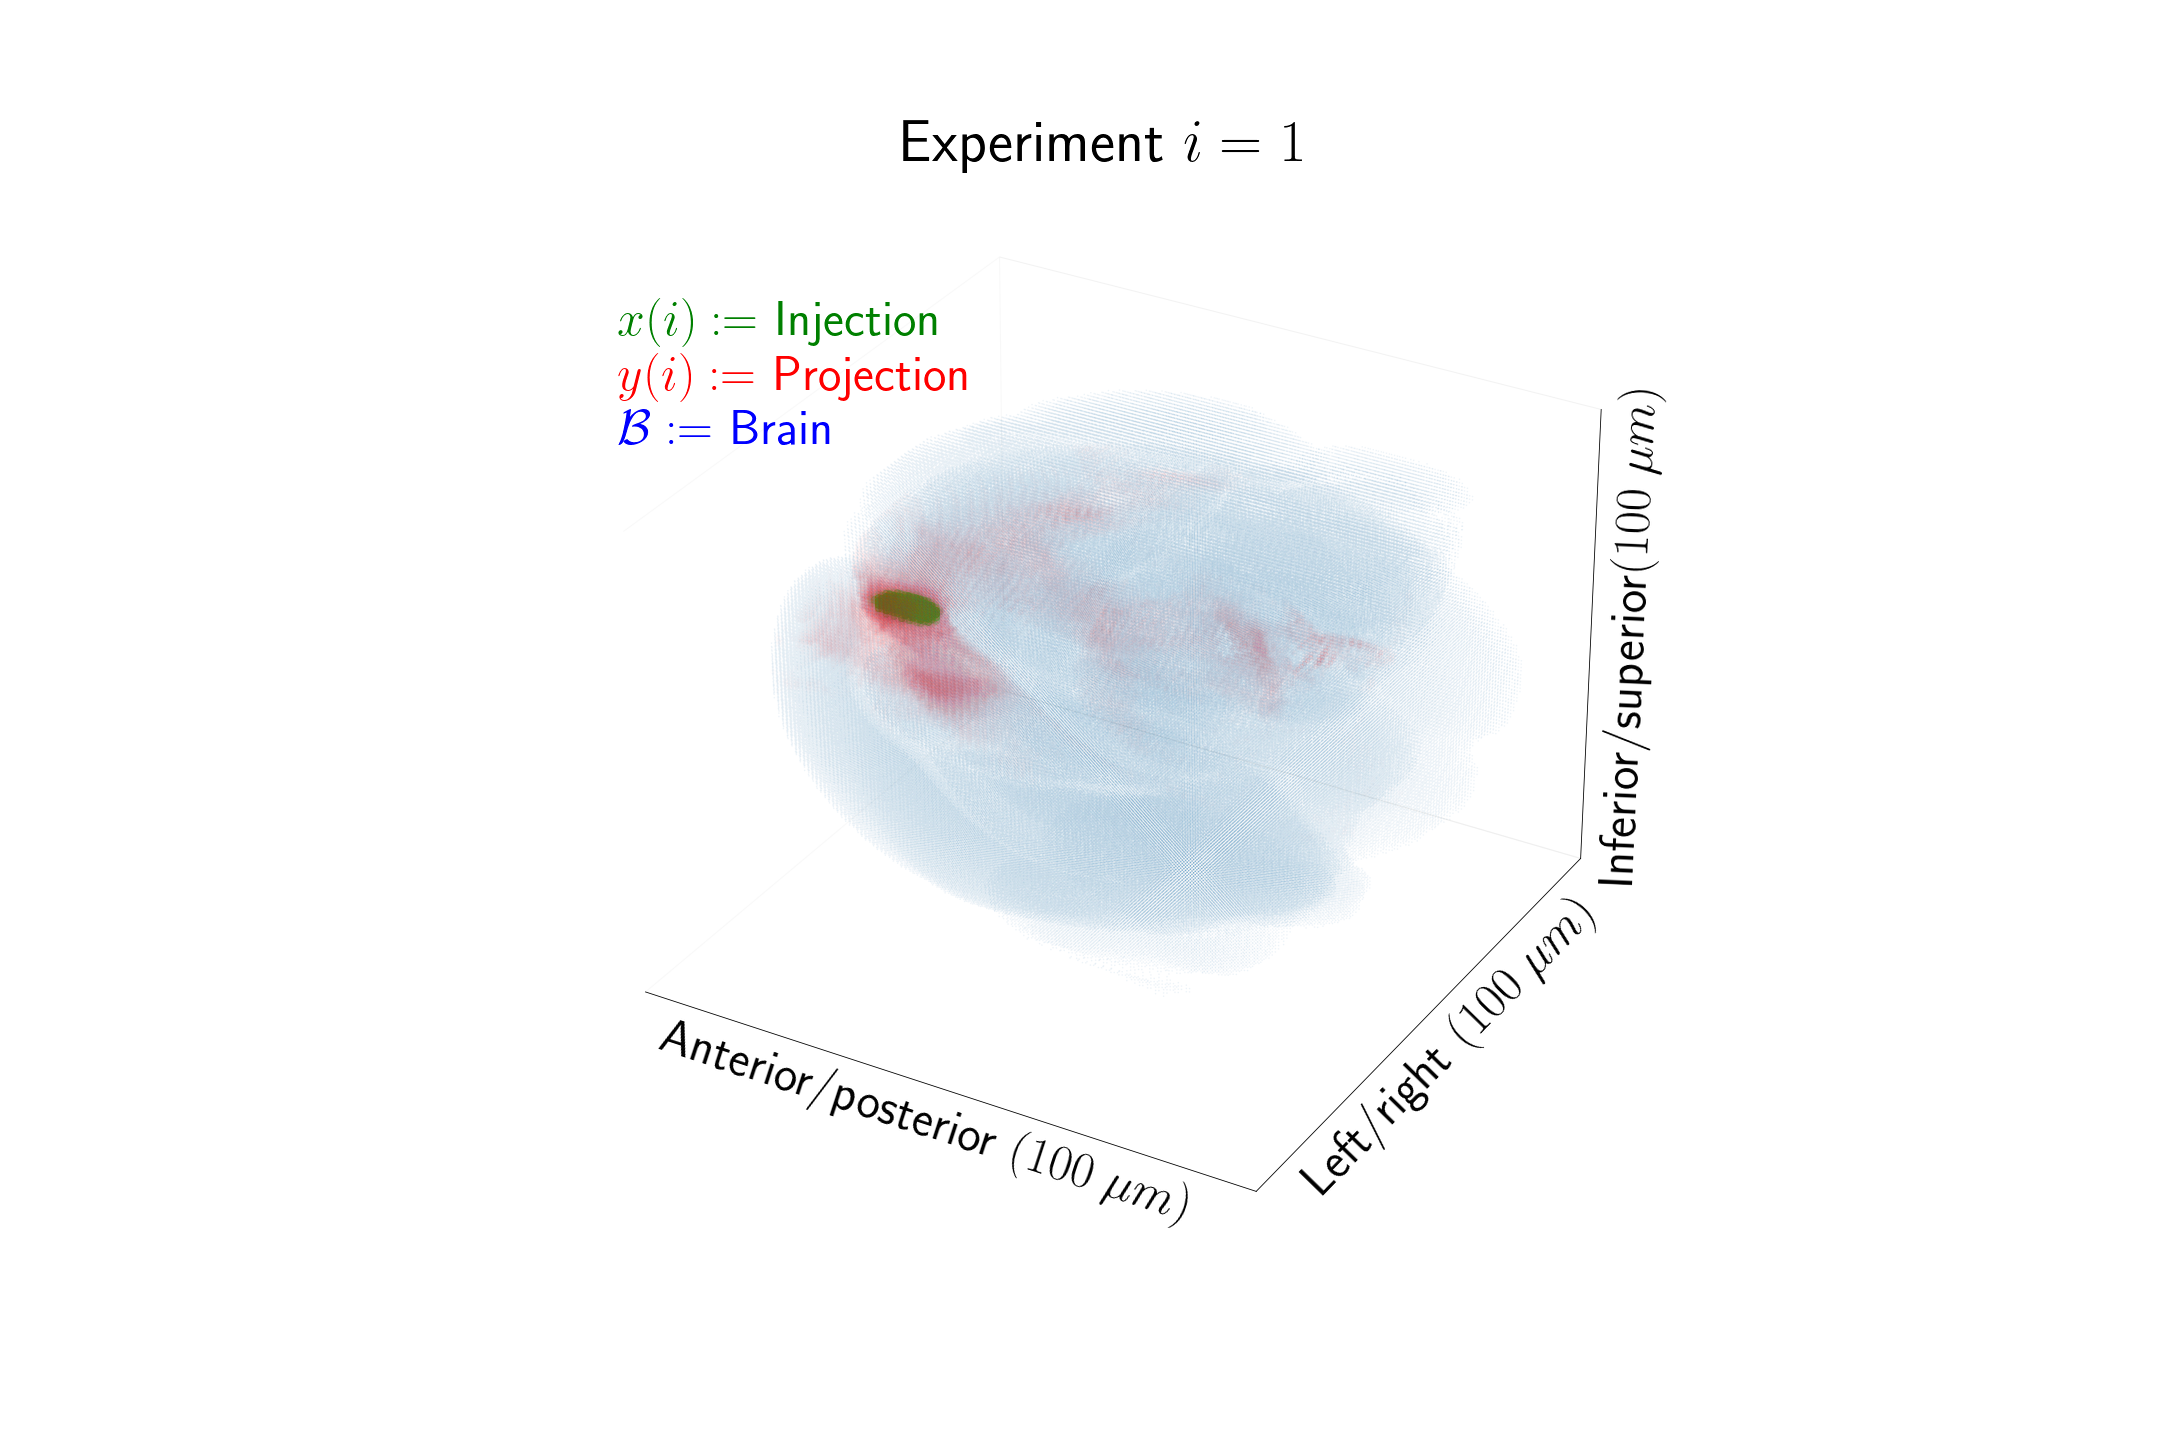
\includegraphics[width=0.4\textwidth]{figs/inj_proj_figure_v2.png}}
\subfloat[]{
\label{fig:segment}
    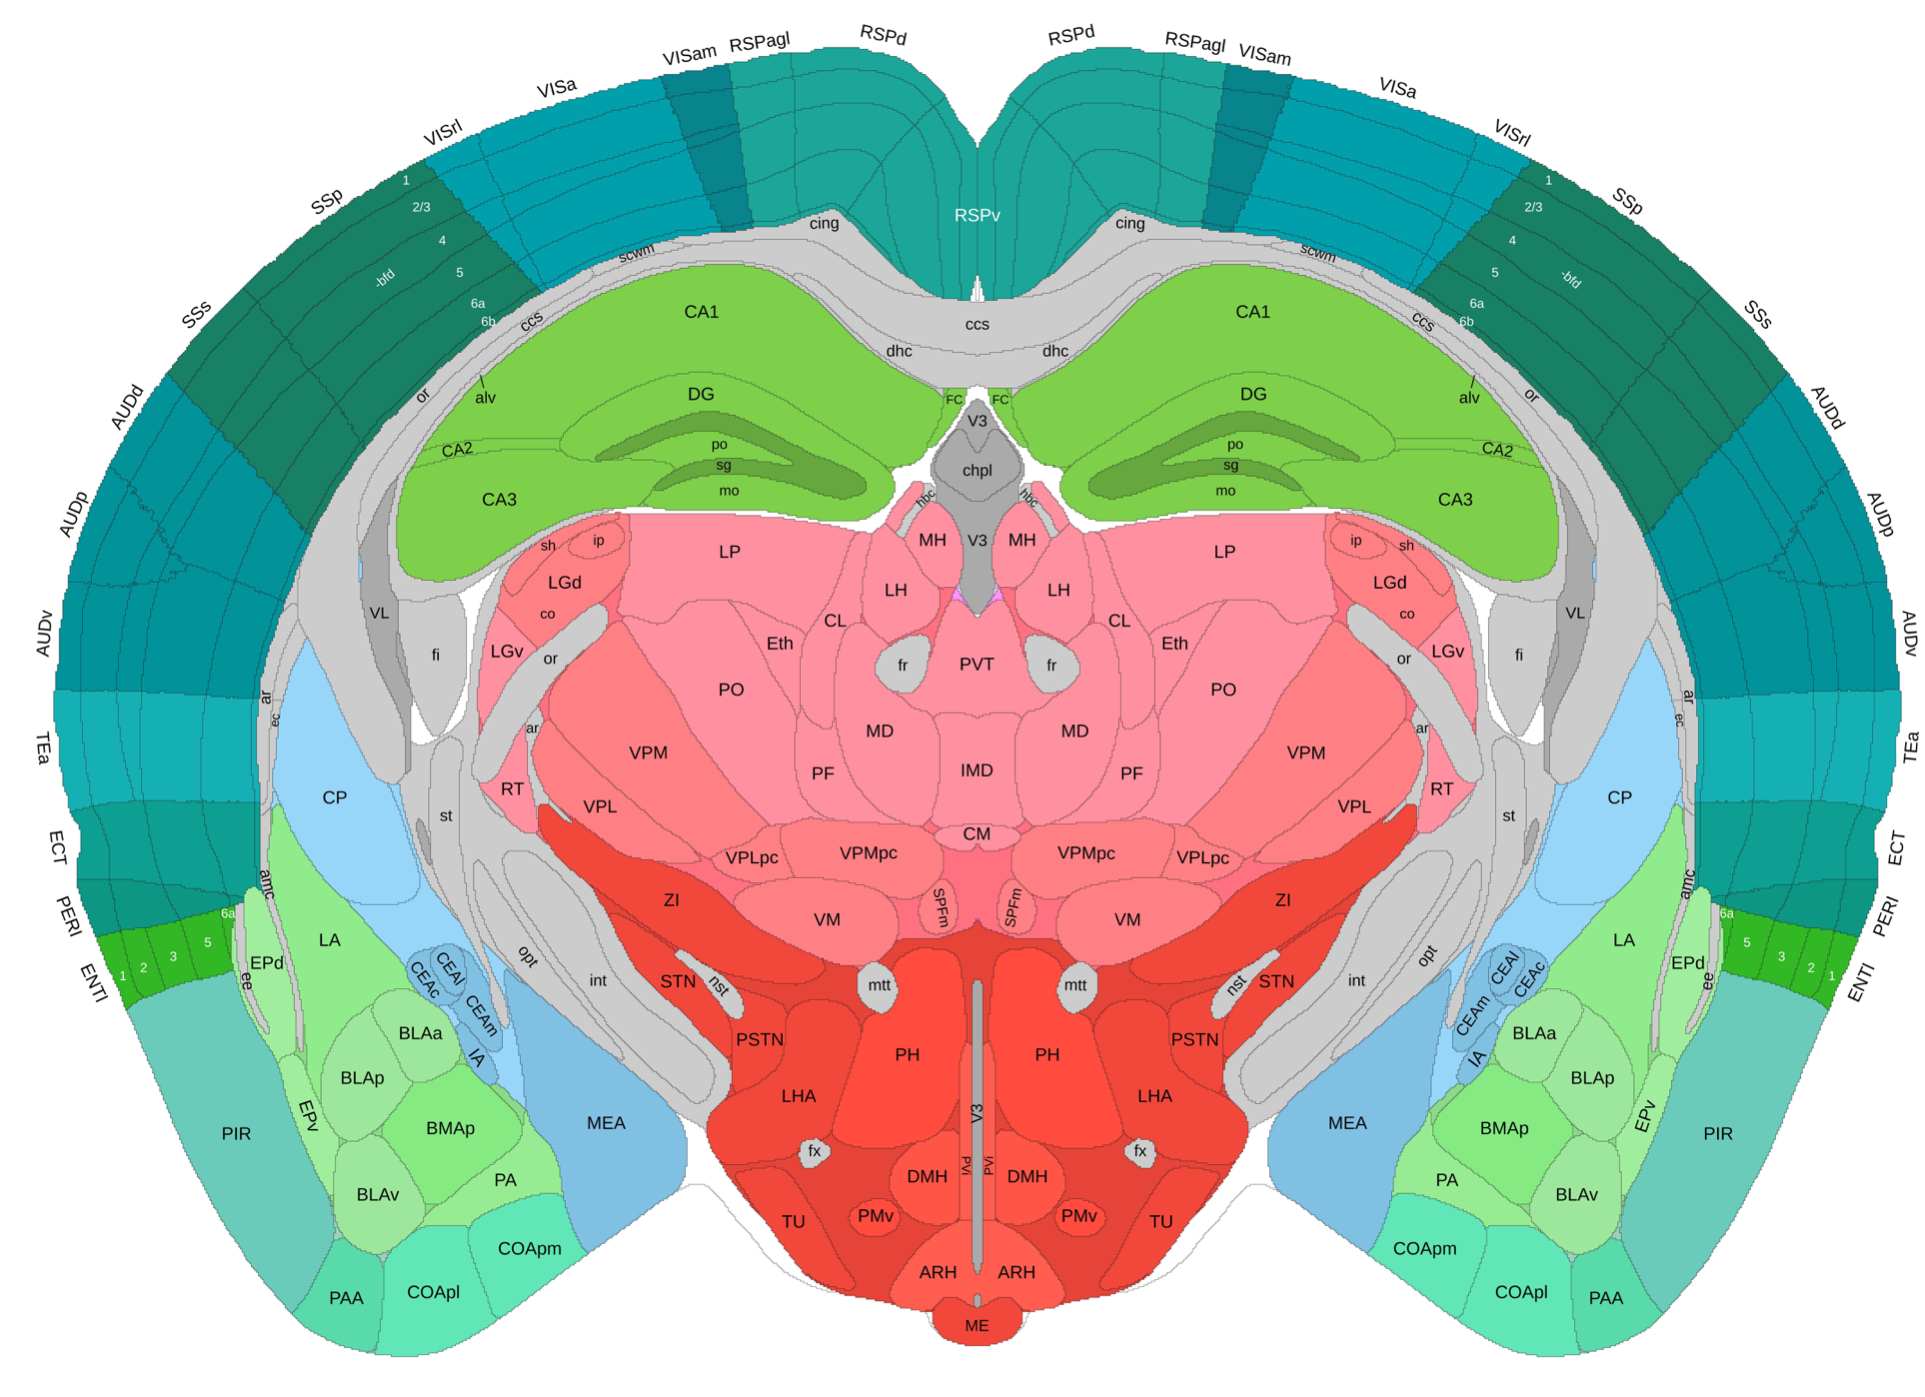
\includegraphics[width=0.3\textwidth]{figs/fig1c.png}}
    \newline
 \subfloat[]{
 \label{fig:ontology}
    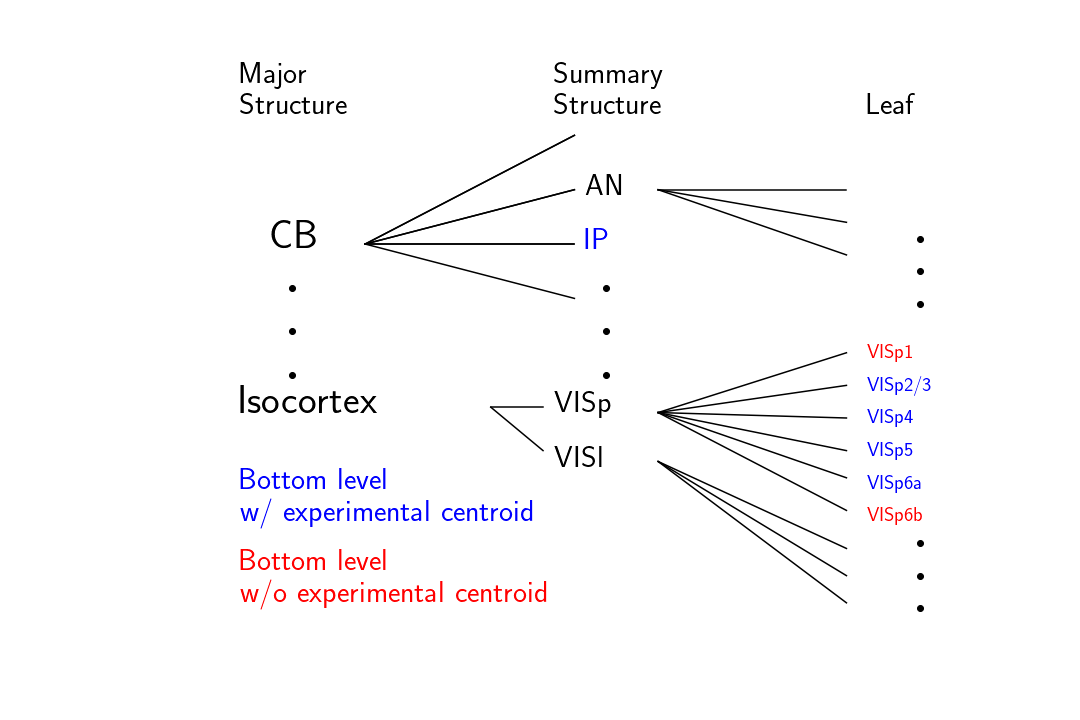
\includegraphics[width=0.35\textwidth]{figs/ontologyfigure.png}}
\subfloat[]{
 \label{fig:top}
    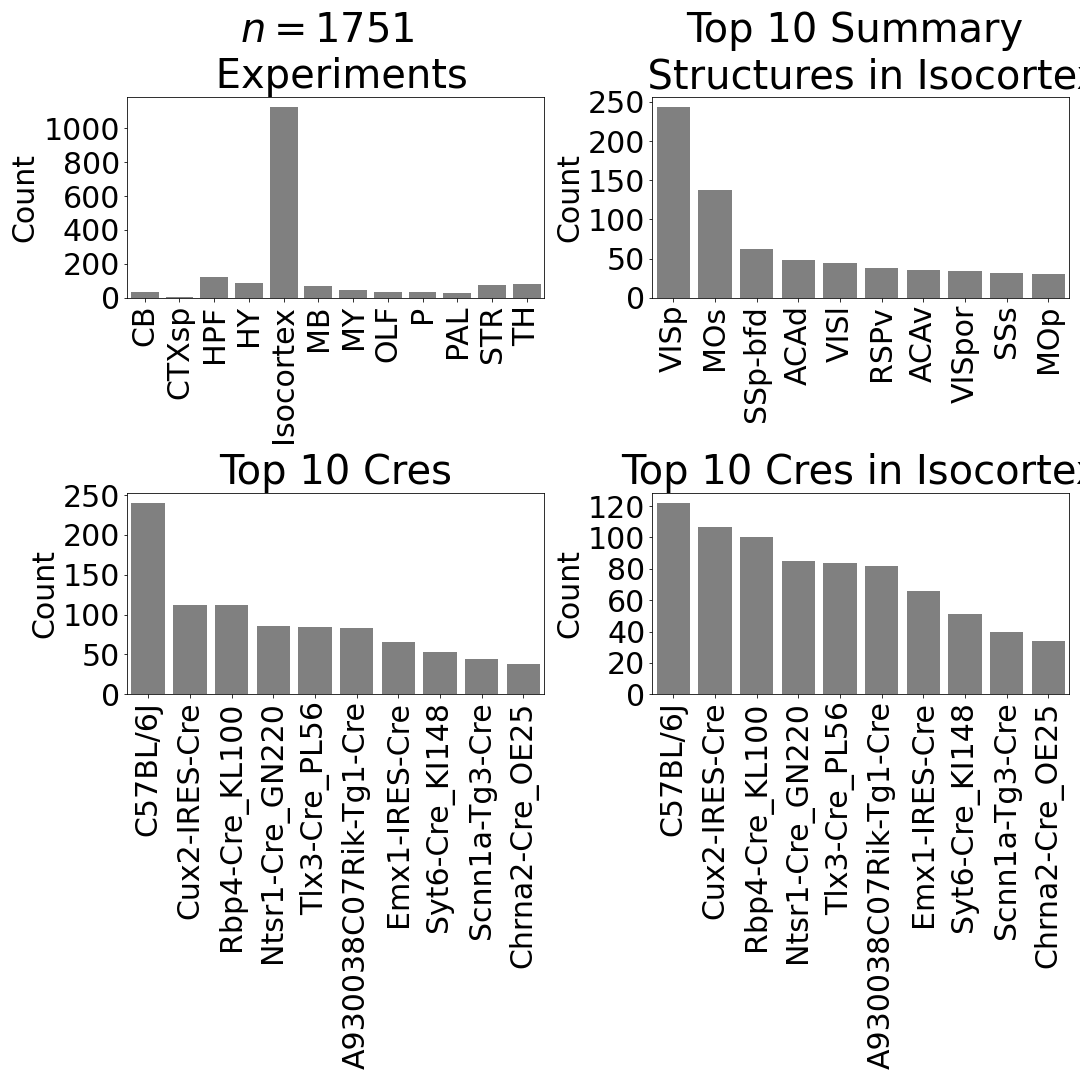
\includegraphics[width=0.35\textwidth]{figs/datasummary.png}}
\subfloat[]{
 \label{fig:combos}
    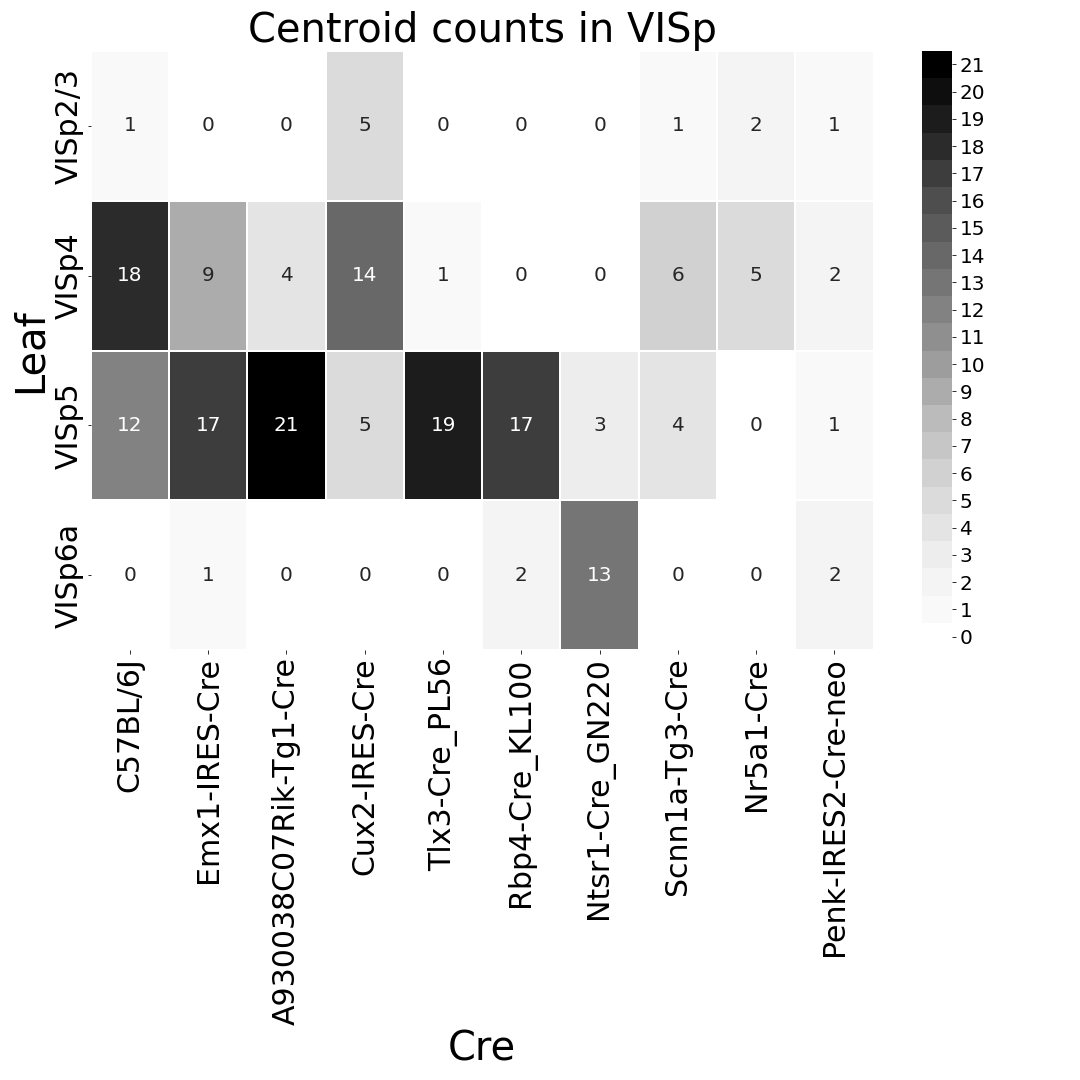
\includegraphics[width=0.35\textwidth]{figs/visp_counts.png}}   
    \caption{Experimental setting.  \ref{fig:mouse}  For each experiment, a potentially Cre-recombinase promoted GFP-expressing transgene casette is transduced after stereotaxic injection into a Cre-driver mouse, followed by two-photon tomography imaging. \ref{fig:injproj} An example of the segmentation of projection and injection for a single experiment. Within each assayed brain (blue), injection (green) and projection (red) areas are determined via histological analysis and alignment to the Allen Common Coordinate Framework (CCF).   \ref{fig:segment} Example of structural segmentation within a horizontal plane. \ref{fig:ontology} Explanation of nested structural ontology highlighting various levels of structural ontology.  Lowest-level (leaf) structures are colored in blue, and structures containing an injection centroid are colored in red. \ref{fig:top}  Abundances of Cre-lines and structural injections. \ref{fig:combos}  Co-occurrence of layer-specific centroids and Cre-line within VISp}
    \label{fig:data}
\end{figure}

\newpage
%\subsection{Mice}
%\skcomment{Experiments involving mice were approved by the Institutional Animal Care and Use Committees of the Allen Institute for Brain Science in accordance with NIH guidelines.}
%\smcomment{such text goes separately in a form somewhere}

\subsection{Data}

Our dataset $\mathcal D$ consists of $n=1751$ publicly available murine viral-tracing experiments from the Allen Brain Connectivity Atlas.
Figure \ref{fig:mouse} summarizes the multistage experimental process used to generate this data.
In each experiment, a GFP-labelled transgene casette with a potentially Cre-inducible promoter is injected into a particular location in a Cre-driver mouse.
This causes fluorescence that depends on the localization of Cre-recombinase expression within the mouse.
While frequently this localization corresponds to a specific cell-type, it can also correspond to a combination of cell-types.
In wild-type mice injected with non-Cre specific promoters, fluorescence is observed in all areas projected to from the injection site, regardless of cell-type.
%Thus, we use the term cell class to describe the neurons targeted by a specific combination (or absence) of transgene and mouse-line. 
Thus, we use the term cell class to describe neurons expressing cre in a specific mouse line.
This is the notion of cell-type specificity that we model.

The fluorescent signal imaged after injection is aligned into the Allen Common Coordinate Framework (CCF) v3, a three-dimensional idealized model of the brain that is consistent between animals.
This imaging and alignment procedure (described in detail in \citep{Harris2019-mr}) records fluorescent intensity discretized at the $100 \; \mu$m \textit{voxel} level. 
Given an experiment, this image is histologically segmented into \textit{injection} and \textit{projection} areas corresponding to areas containing somas, dendrites and axons or exclusively axons of the transfected neurons.
An example for a single experiment is given in Figure \ref{fig:injproj}.

Our goal is the estimation of \textit{structural connectivity} from one structure to another.
A visual depiction of this structural regionalization for a slice of the brain is given in Figure \ref{fig:segment}.
For different areas of the brain, the Allen Brain Atlas contains different depths of regionalization.
We denote these levels as Major Structures, Summary Structures, and Leafs.
As indicated in Figure \ref{fig:ontology}, the dataset used to generate the connectivity model reported in this paper contains certain combinations of structure and cell class $(v,s)$ frequently, and others not at all.
A summary of the most frequently assayed cell classes and structures is given in Figures \ref{fig:top} and \ref{fig:combos}.
Since users of the connectivity matrices may be interested in particular combinations, or interested in the amount of data used to generate a particular connectivity estimate, we present this information about all experiments in Supplemental Section \ref*{supp_sec:data}.

A cell-class specific neural connectivity is a function $f:  \mathcal V \times \mathbb R^3 \times \mathbb R^3 \to \mathbb R_{\geq 0}$ giving the directed connection of a particular cell class from a one position in the brain to another.
However, what we will actually estimate are structural connectivities defined with respect to a set of $S$ source regions $\mathcal S := \{ s\} $, $T$ target regions $\mathcal T := \{ t \}$, and $V$ cell classes $\mathcal V := \{v\}$.
In contrast to \citet{Knox2019-ot}, which only uses wild type C57BL/6J mice, these experiments utilize $V = 114$ different Cre-lines. 
We generally consider $S = 564$ leaf sources and $T = 1123$ leaf targets, where $559$ are contralateral and 5 are  mediolateral, but other structuralizations could be used.

We preprocess our data in several ways.
We discretize fluorescent signals like injections and projections into $100 \mu m^3$  \textbf{voxels}.
Given an experiment $i$, we represent injections and projections as maps $x(i),y(i) : \mathcal B \to \mathbb R_{\geq 0}$, where $\mathcal B \subset [1:132] \times [1:80] \times [1:104]$ corresponds to the subset of the $(1.32 \times 0.8 \times 1.04)$ cm rectangular space occupied by the standard mouse brain.
As an abuse of notation, a structure $s$ then contains $|s|$ voxels at locations $\{l_{s_j} \in \mathbb R^3\}$, and similarly for targets.
We calculate injection centroids $c(i) \in \mathbb R^3$ and regionalized projections $y_{\mathcal T} (i) \in \mathbb R^{T} $ giving the sum of $y(i)$ in each region.
In contrast to \citet{Knox2019-ot}, we generally $l1$ normalize the projection vectors.
This accounts for differences in the cre-driven expression of eGFP via the various transgene promoters.
However, we also for completeness include models of projections normalized by injection signal.
A detailed mathematical description of these steps, including data quality control, is given in Supplemental Section \ref{supp_sec:dp}.

\newpage

\subsection{Modeling Structural Connectivity}
We define
\begin{align*}
&\text{\textit {structural connectivity strength} } \mathcal C : \mathcal V \times \mathcal S \times \mathcal T \to \mathbb R_{\geq 0}  \text{ with } \mathcal C(v,s,t) = \sum_{l_{s_j} \in s} \sum_{l_{j'} \in  t} f(v,l_{j},l_{j'}), \\
&\text{\textit {normalized structural connectivity strength} } \mathcal C^S : \mathcal V \times \mathcal S \times \mathcal T \to \mathbb R_{\geq 0}  \text{ with } \mathcal C^S(v,s,t) = \frac{1}{|s|} \mathcal C(v,l_{j},l_{j'}), \\
%&\text{\textit {normalized structural projection density} } \mathcal C^D : \mathcal V \times \mathcal S \times \mathcal T \to \mathbb R_{\geq 0} \text{ with } \mathcal C^D(v,s,t) = \frac{1}{| s | | t|}\mathcal C(v,l_{j},l_{j'}).
\end{align*}
These are the total strength and average strength from source to target regions for each class \skcomment{no density}.
Since the normalized strength is computable from the strength via a fixed normalization, our main statistical goal is to estimate $\mathcal C (v,s,t) $ for all $v, s$ and $t$.% and density are
We call this estimator $\widehat { \mathcal C } $.

Construction of such an estimator raises the questions of what data to use for estimating which connectivity, how to featurize the dataset, what statistical estimator to use, and how to reconstruct the connectivity using the chosen estimator.
Mathematically, we represent these considerations as 
\begin{align}
\label{eq:estimator}
\widehat { \mathcal C }(v,s,t) = f^* (\widehat f (f_*( \mathcal D(v,s,t))).
\end{align}
This makes explicit the data featurization $f_{*}$, statistical estimator $\widehat f$, and any potential subsequent transformation $f^*$ such as summing over the source and target regions.
Denoting $ \mathcal D$ as a function of $v,s,$ and $t$ reflects that different data may be used to estimate different connectivities.
Table \ref{tab:estimators} reviews estimators used for this data-type used in previous work, as well as our two main extensions: the Cre-NW and \textbf{Expected Loss} (EL) models.
Additional information on these estimators is given in Supplemental Section \ref{supp_sec:estimators}.

\begin{table}[H]
    \centering
    \begin{tabular}{c|c|c|c|c|}
        Name & $f^*$ & $\widehat f$&  $ f_*$ & $\mathcal D(v,s)$ \\
        \hline
        %Leaf-mean & & & & \\
        NNLS \citep{Oh2014-kh} & $\widehat f (S)$ & \nnls(X,Y) & $X= x_{\mathcal S},Y = y_{\mathcal T}$ & $ I_m / I_m$ \\
        NW \citep{Knox2019-ot} &$ \sum_{l_s \in s} \widehat f (l_s)$ & \nw(X,Y)  & $X = c, Y = y_{\mathcal T}$ & $I_m /I_m$ \\
        %Cre-leaf-mean & & & & \\
        Cre-NW& $\sum_{l_s \in s} \widehat f(l_s)$ & \nw(X,Y) & $X= c, Y = y_{\mathcal T}$  &$ (I_s \cap I_v) / I_m$ \\
        Expected Loss (EL) & $\sum_{l_s \in s} \widehat f (s)$ & $\el(X,Y,v)$ & $X= c, Y = y_{\mathcal T}, v$  &$I_s / I_m$
    \end{tabular}
    \caption{Estimation of $\mathcal C$ using connectivity data.
    The regionalization, estimation, and featurization steps are denoted by $f^*, \widehat f,$ and  $f_*$, respectively.
    The training data used to fit the model is given by $I$.
    We denote experiments with centroids in particular major brain divisions and leafs as $I_m$ and $I_s$, respectively.
    Data $I_s / I_m$ means that, given a location $l_s \in s \in m$, the model $\widehat f$ is trained on all of $I_m$, but only uses $I_s$ for prediction. \smcomment{add more description of NNLS, NW, etc}
    }
    \label{tab:estimators}
\end{table}

Our contributions have several differences from the previous methods.
In contrast to the non-negative least squares \citep{Oh2014-kh} and Nadaraya-Watson  \citep{Knox2019-ot} estimators that take into account $s$ and $t$, but not $v$, our new estimators specifically account for cell class.
The Cre-NW estimator only uses experiments from a particular class to predict connectivity for that class, while the EL estimator shares information between classes within a structure.
A detailed mathematical description of our new estimator is given in Appendix \ref{supp_sec:el}.
This estimator takes into account two types of covariate information about each experiment: the centroid of the injection, and the Cre-line.
Like the NW and Cre-NW estimator, the EL estimator generates predictions for each voxel in a structure, and then sums them together to get the overall connectivity.
However, in contrast to these alternative approaches, when predicting the projection pattern of a certain cell-class at a particular location, the EL estimator weights the average behavior of the class in the structure containing the location in question against the locations of the various proximal experiments. 
Thus, nearby experiments with similar Cre-lines can help generate the prediction, even when there are few nearby experiments of the cell-class in question.

\newpage

\subsection{Model evaluation}

We select optimum functions from within and between our estimator classes using {\textit leave-one-out cross validation}, in which the accuracy of the model is assessed by its ability to predict experiments excluded from the training data. %in leave-one-out cross-validation.
Equation \ref{eq:estimator} includes a deterministic step $f^*$ included without input by the data.
The performance of $\widehat {\mathcal C (v,s,t)}$ is thus determined by performance of $\widehat f (f_*(\mathcal D(v,s)))$.
Furthermore, we can represent $f$ as $f_{\mathcal T}: \mathbb R^3 \to \mathbb R_{\geq 0}^T$ giving the structural connection strength at a given location.
This is the predictand we evaluate. 

Another question is what combinations of $v, s, $ and $t$ to generate a prediction for.
Our EL and Cre-NW models are leaf specific.
They only generate predictions for cell classes in leafs where at least one experiment with a Cre-line targeting that class has a centroid.
To compare our new estimators accurately with less-restrictive models such as used in \citet{Knox2019-ot}, we therefore restrict restrict to the smallest set of evaluation experiments suggested by any of our models: virus-leaf combinations that are present at least twice. 
The sizes of these evaluation sets are given in Supplemental Section \ref{supp_sec:model-evaluation}.

We use weighted $l2$-loss to evaluate these predictions.
\begin{align*}
\text{l2-loss } \ell (y_{\mathcal T}(i)),\widehat {y_{\mathcal T}(i))}) &:=   \| y_{\mathcal T} (i)) - \widehat {y_{\mathcal T}(i))} \|_2^2. \\
\text{weighted l2-loss } \mathcal L ( \widehat {f(f_*)}) &:= \frac{1}{|\{s,v\}|} \sum_{s,v \in \{\mathcal S,\mathcal V\}} \frac{1}{ |I_{s} \cap I_v |} \sum_{i \in (I_{s} \cap I_v ) } \ell (y_{\mathcal T}(i)), \hat f_{\mathcal T} (f_*(\mathcal D(v,s) \setminus i)) .
\end{align*}
This is a somewhat different loss from \citet{Knox2019-ot}, both because of the normalization of projection, and because of the increased weighting of rarer combinations of $s$ and $v$ implicit in the loss.
Since the number of parameters fit is very low (at least two orders of magnitude) relative to the size of the evaluation set, we do not make use of a formal validation-test split.  %skcomment which grows quadratically with the number of experiments removed
As a final modeling step, we establish a lower limit of detection.
The EL model also contains a separate cross-validation step.
These approaches are covered in Supplemental Section \ref{supp_sec:methods_lower}

\newpage

\subsection{Connectivity analyses}

We show neuronal processes underlying our estimated connectome using two types of unsupervised learning.
Our use of heirarchical clustering is standard, and so we do not review it here.
However, our application of non-negative matrix factorization (NMF) to decompose the estimated long-range connectivity into \textit{connectivity archetypes} that linearly combine to reproduce the observed connectivity is novel and technically of some independent interest.
Non-negative matrix factorization refers to a collection of \textbf{dictionary-learning} algorithms for decomposing a non-negatively-valued matrix such as $\mathcal C $ into positively-valued matrices called, by convention, weights $W \in \mathbb R^{S \times q}_{\geq 0}$ and hidden units $H \in \mathbb R^{q  \times T}_{\geq 0}$.
Unlike PCA, NMF specifically accounts for the fact that data are all in the positive orthant.
This $H$ is typically used to identify latent structures with interpretable biological meaning, and the choice of matrix factorization method reflects particular scientific subquestions and probabilistic interpretations. 

Our algorithm is 
\begin{eqnarray*}
\label{eq:nmf}
\nmf(\mathcal C, \lambda, q) := \arg \min_{W, H} \frac{1}{2}\| 1_{d(s,t) > 1500 \mu m} \odot \mathcal C - WH\|_2^2  + \lambda  (\|H \|_1 + \|W \|_1) .
\end{eqnarray*}
For this decomposition we ignore connections between source and and target regions less than  $1500 \mu m$ apart.
This is because short-range projections resulting from diffusion dominate the matrices $\hat {\mathcal C}$, and represent a less-interesting type of biological structure.
We explored different values and set $\lambda = 0.002$ to encourage sparser and therefore more interpretable components.
We use unsupervised cross-validation to determine an optimum $q$, and show the top $15$ stable components.
Stability analysis accounts for the difficult-to-optimize NMF program by clustering the resultant $H$ from multiple replicates.
The medians of the component clusters appearing frequently across NMF replicates are selected as \textbf{connectivity archetypes}.
Details of these approaches are given in Supplementary Sections \ref{supp_sec:matrix_factor_methods} and \ref{supp_sec:matrix_factor_results}.

%Second, we extend the characterization of \citet{Knox2019-ot} on structural differences in short-range projections.
%These are primarily assumed to be due to diffusion, and the diffusion-rate helps to characterize the basic structural anatomy.
%The latter issue is ameliorated by regularization terms to encourage finding vectors around which  $\hat {\mathcal C}$ is clustered.


